\documentclass[border=10pt]{standalone}
\usepackage{pgfplots}
\usepgfplotslibrary{colormaps}
\pgfplotsset{compat=1.18}

\begin{document}
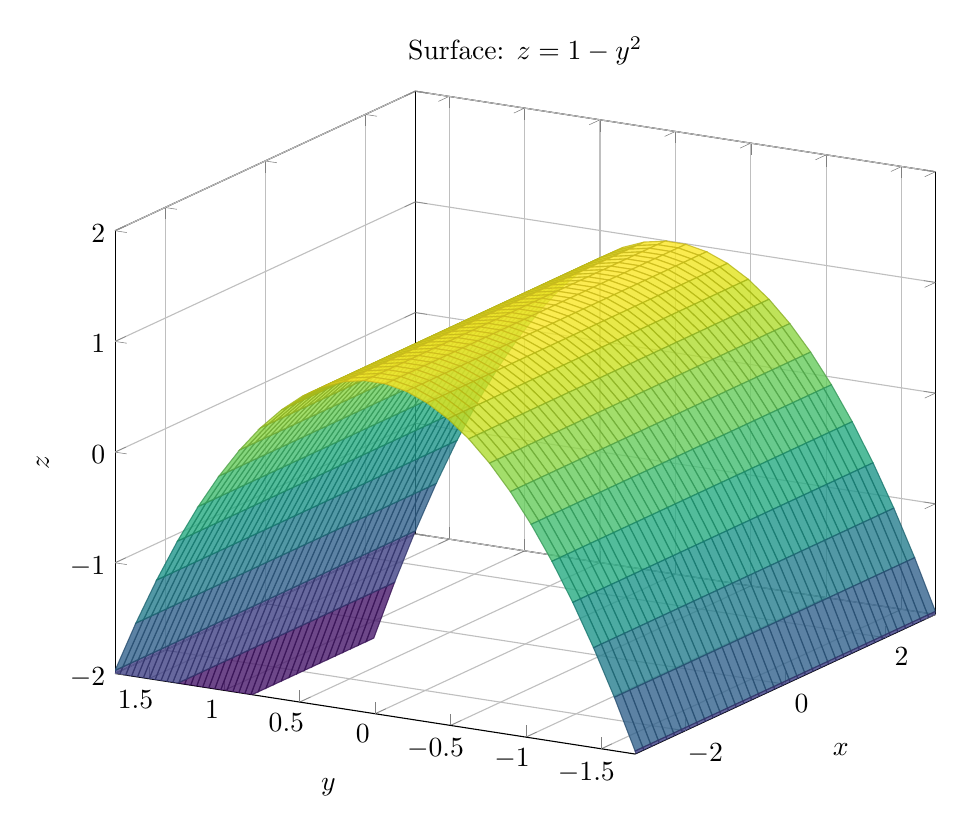
\begin{tikzpicture}
\begin{axis}[
    xlabel={$x$},
    ylabel={$y$},
    zlabel={$z$},
    title={Surface: $z = 1 - y^2$},
    view={-60}{20},
    colormap/viridis,
    grid=major,
    width=12cm,
    height=10cm,
    zmin=-2,
    zmax=2,
]
\addplot3[
    surf,
    domain=-3:3,
    y domain=-2:2,
    samples=40,
    samples y=30,
    opacity=0.8,
] {1 - y^2};
\end{axis}
\end{tikzpicture}
\end{document}